\section{Introduction}
	\subsection{Artificial Neural Networks}
		\subsubsection{Motivation From Biology}
		The brain is a critical component in our body that enables learning. It has about 10 billion interconnected neurons. A neuron receives input from other neurons from its synapses. Sum of input happens, and when the sum exceeds a particular threshold, the neuron sends an electrical spike to another neuron(s) through the axon. 

		\subsubsection{Perceptron}
		Perceptron is an algorithm in machine learning for supervised learning of binary classifiers, i.e., a function to determine the class in which the input vector belongs.

\begin{figure}
	\centering
		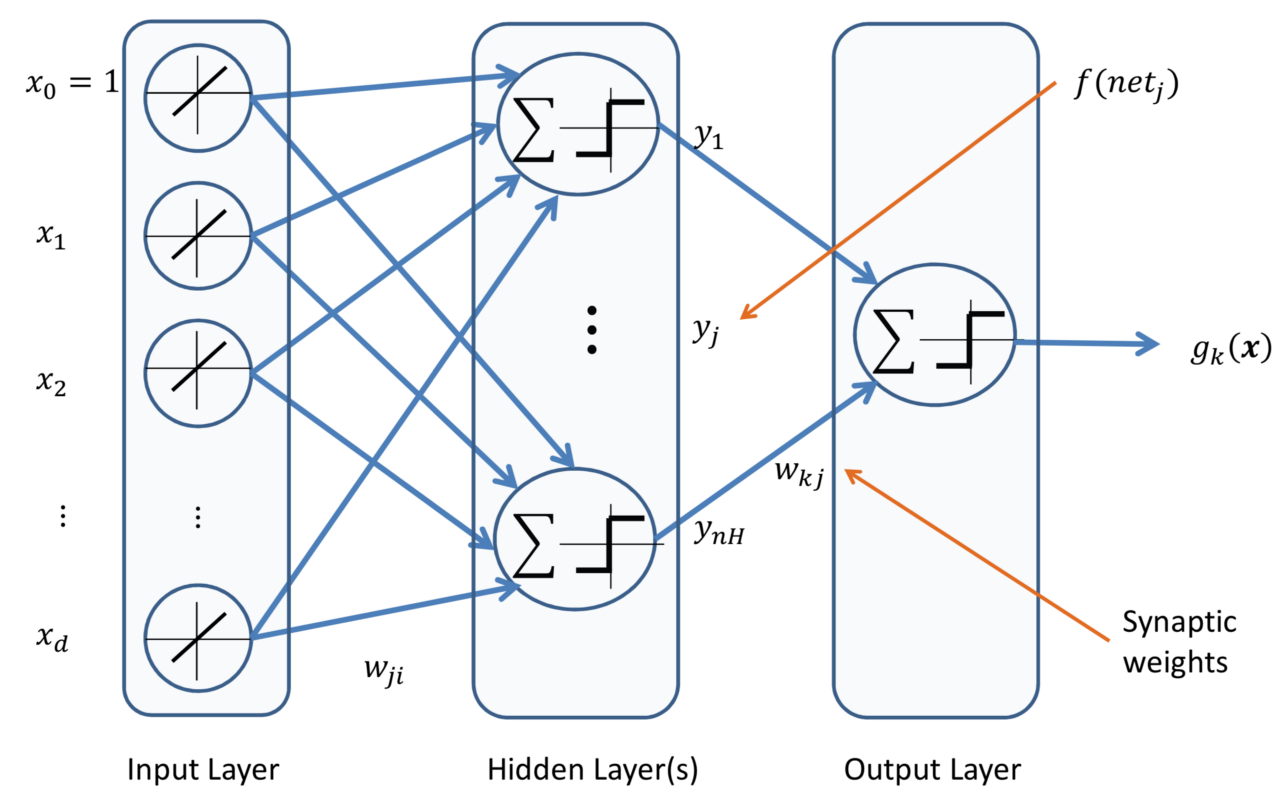
\includegraphics[width=0.6\linewidth]{images/introduction_neural.png}
	\caption{An artificial neuron with one input, one hidden and one output layer.}
	\label{fig:introduction_fig}
	\end{figure}

		\subsubsection{Towards Neural Nets}
A basic artificial neural network is a natural extension to perceptron. We can say that a basic neural network is a multi-layer perceptron called a feed-forward neural network.  An Artificial Neuron Network (ANN), popularly known as Neural Network is a computational model based on the structure and functions of biological neural networks. It is like an artificial human nervous system for receiving, processing, and transmitting information in terms of Computer Science. Basically, there are 3 different layers in a neural network, input layer, hidden layer and output layer. An ANN would contain :
		\begin{itemize}
			\item Hidden Layers
			\item Bias Units
			\item Neurons(input, output and perceptron)
			\item Synaptic weights
		\end{itemize}

	\subsection{Deep Neural Networks}
	Deep learning (also known as deep structured learning) is part of a broader family of machine learning methods based on artificial neural networks with representation learning. Learning can be supervised, semi-supervised or unsupervised.	\cite{bengio2013representation,schmidhuber2015deep}

Deep learning architectures such as deep neural networks, deep belief networks, recurrent neural networks and convolutional neural networks have been applied to fields including computer vision, speech recognition, natural language processing, audio recognition, social network filtering, machine translation, bioinformatics, drug design, medical image analysis, material inspection and board game programs, where they have produced results comparable to and in some cases surpassing human expert performance.\cite{krizhevsky2012imagenet}

Artificial neural networks (ANNs) were inspired by information processing and distributed communication nodes in biological systems. ANNs have various differences from biological brains. Specifically, neural networks tend to be static and symbolic, while the biological brain of most living organisms is dynamic (plastic) and analog.

\begin{figure}[htbp]
	\centering
		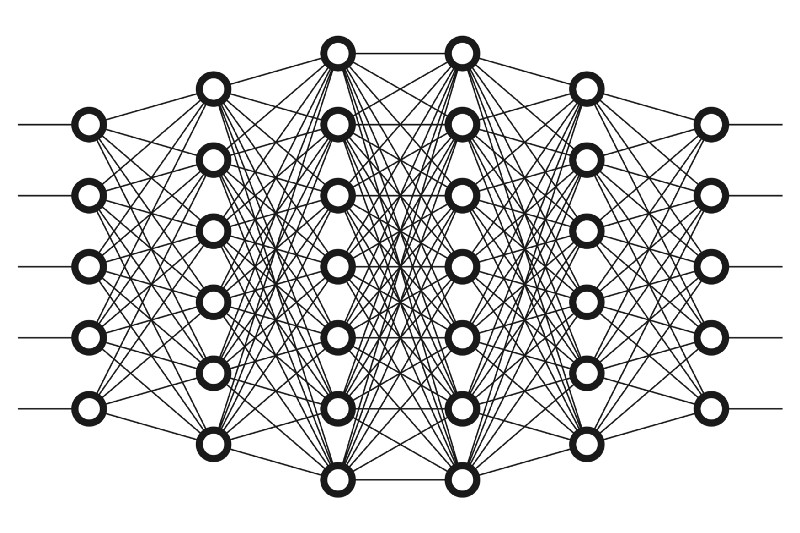
\includegraphics[width=0.6\linewidth]{images/deep_neural_network.jpeg}
	\caption{An deep neuron network with one input, four hidden and one output layer.}
	\label{fig:deep_neural_network}
	\end{figure}

Most modern deep learning models are based on artificial neural networks, specifically, Convolutional Neural Networks (CNN)s, although they can also include propositional formulas or latent variables organized layer-wise in deep generative models such as the nodes in deep belief networks and deep Boltzmann machines.\cite{bengio2009learning}

In deep learning, each level learns to transform its input data into a slightly more abstract and composite representation. In an image recognition application, the raw input may be a matrix of pixels; the first representational layer may abstract the pixels and encode edges; the second layer may compose and encode arrangements of edges; the third layer may encode a nose and eyes; and the fourth layer may recognize that the image contains a face. Importantly, a deep learning process can learn which features to optimally place in which level on its own. (Of course, this does not completely eliminate the need for hand-tuning; for example, varying numbers of layers and layer sizes can provide different degrees of abstraction.)\cite{bengio2013representation,lecun2015deep}
